\documentclass[11pt,a4paper]{ctexart}
\usepackage{indentfirst} %首行缩进
\usepackage[hyperfootnotes=true]{hyperref}
\hypersetup{%
pdftitle = {Ubuntu 16.04 + NVIDIA GeForce GTX 1080Ti 配置TensorFlow-GPU 1.6.0},
	pdfauthor = {万震(wanzhen@cqu.edu.cn)},
	linktoc=all,
	bookmarksnumbered=true,
	bookmarksopen=true,
	bookmarksopenlevel=3,
	breaklinks=true,
	colorlinks=true,
	allcolors=blue,
	urlcolor=magenta,
	plainpages=false,
	pdfborder=0 0 0}
\usepackage{amsmath,amsthm,verbatim,amssymb,amsfonts,amscd, graphicx}
\graphicspath{{figure/}} % 定义所有的图片文件在 figures 子目录下

\usepackage{xeCJK} %设置中文字体
\setCJKmainfont{SimSun} %xeCJK宏包下设置全局默认中文字体

\usepackage{fontspec}  %设置英文字体
\setmainfont{Palatino Linotype}






\begin{document}
\title{Ubuntu 16.04$ \times$86\_64 + NVIDIA GeForce GTX 1080Ti +  CUDA 9.0 + cuDNN 7.0配置TensorFlow-GPU 1.6.0 }  
\author{\kaishu\Large 万\ 震\\ \href{mailto:wanzhen@cqu.edu.cn}{wanzhen@cqu.edu.cn}}
\date{2018年3月18日}
\maketitle

TensorFlow 有 CPU和 GPU两个版本,GPU版本需要NVIDIA的CUDA 和 cuDNN 支持,CPU版本不需要\footnote{\url{https://github.com/tensorflow/tensorflow/releases}}。CUDA(Compute Unified Device Architecture)是显卡厂商NVIDIA 推出的运算平台。 $CUDA^{TM}$是一种由 NVIDIA 推出的通用并行计算架构,该架构使 GPU 能够解决复杂的计算问题。它包含了CUDA 指令集架构(ISA)以及 GPU 内部的并行计算引擎。NVIDIA CUDA® Deep Neural Network library (cuDNN) 是NVIDIA 专门针对深度神经网络(Deep Neural Networks)中的基础操作而设计基于 GPU 的加速库,其被广泛用于各种深度学习框架,例如TensorFlow, Caffe, Theano, Torch, CNTK等。cuDNN 为深度神经网络中的标准 流 程 ( forward and backward convolution, pooling, normalization, and activation layers)提供了高度优化的实现方法\footnote{\url{https://developer.nvidia.com/cuda-toolkit}}。

本教程配置环境为:
\vspace{-0.3cm}
\begin{itemize}
\item Ubuntu 16.04$ \times$86\_64  LTS、NVIDIA GeForce GTX 1080Ti 
\item CUDA 9.0 、 cuDNN 7.0、TensorFlow-GPU 1.6.0
\end{itemize}
文中首先介绍了配置之前的相关准备工作,包括查看NVIDIA显卡型号和对应驱动是否安装、验证NVIDIA显卡是否支持CUDA、修改ubuntu默认python版本、安装pip并升级、完全卸载旧版本CUDA;其次介绍了CUDA 9.0 、 cuDNN 7.0以及libcupti-dev 库的安装;再次介绍了环境变量的配置、测试 CUDA 9.0 和 cuDNN 7.0 的安装情况;随后介绍了配置 TensorFlow-GPU 环境并测试其安装情况;最后介绍了导入tensorflow出现的常见问题及其解决办法。

本文所述方法适用于以上环境但所体现的思想不限于此种组合,读者可根据本教程配置类似组合。

% 准备工作
\section{准备工作}
\subsection{查看NVIDIA显卡型号和相应驱动是否安装}
快捷键Ctrl+Alt+T调出终端,输入如下命令:
\begin{center}
\$ nvidia-smi
\end{center}
查看NVIDIA显卡属性,若本机驱动已安装,则显示类似下图信息。

\begin{figure}[h]
\begin{center}
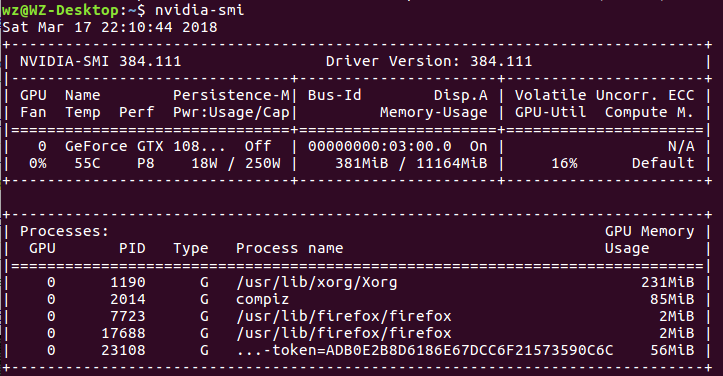
\includegraphics[width=0.9\textwidth]{NIVIDIA_Info} 
\end{center}
\end{figure}
\vspace{-0.5cm}
从上图第一行可以看出本机安装的NVIDIA显卡驱动版本为384.111;第二行中可以看出本机NVIDIA显卡名字为:GeForce GTX 1080,GPU编号为0。

若NVIDIA显卡驱动未安装,则上述命令无法查询以上信息,可以使用如下命令进行驱动安装:
\begin{center}
\$ sudo ubuntu-drivers autoinstall 
\end{center}
然后再次使用命令\$ nvidia-smi 查看NVIDIA显卡驱动是否已经安装;或者进入系统设置,点击底部的详细信息,若概况栏目正确显示出本机CPU、GPU信息则表明驱动已经正确安装,若上述操作均已顺利执行,但概况栏目仍未正确显示出本机CPU、GPU信息,则重启Ubuntu系统即可。


\subsection{验证NVIDIA显卡是否支持CUDA}
点击 \url{https://developer.nvidia.com/cuda-gpus} 进入 NVIDIA GPUs 页面,根据本机NVIDIA显卡型号进入相应列表查看其是否在列,同时查看其是否满足Compute Capability $\geq$ 3.0。若在列且满足Compute Capability $\geq$ 3.0,那么恭喜你,请继续阅读下文;否则你懂的。
%\begin{figure}[h]
%\begin{center}
%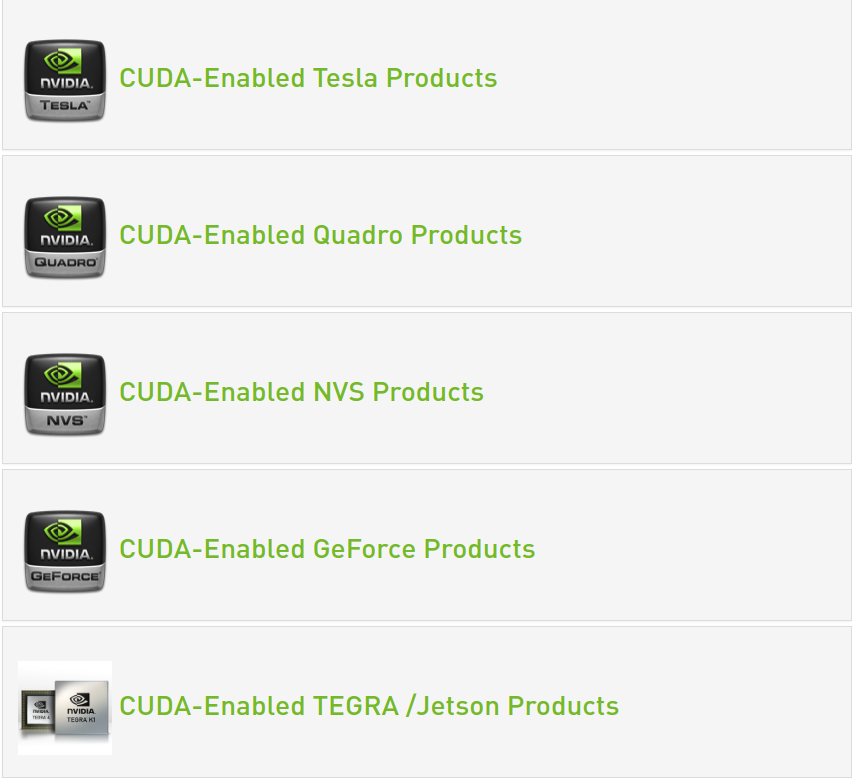
\includegraphics[width=0.9\textwidth]{CUDA_GPUs} 
%\end{center}
%\end{figure}
%\vspace{-0.5cm}

\subsection{安装Python 3.6/3.5 $\times $64 }
由于Ubuntu 16.04 LTS版本自带Python 2.7 和Python 3.5,为后续顺利搭建TensorFlow-GPU环境,请务必安装Python 3.5及其以上版本,当然系统自带的Python 3.5版本足以满足要求,本着“少折腾”原则,可以“就地取材”使用系统自带Python 3.5。

但是,Ubuntu 16.04 LTS默认使用Python 2.7(可在终端输入:python -V 查看本机默认采用的python 版本,然后进入/usr/local/lib 查看当前系统中已安装的python版本;若有需要,可使用命令sudo apt-get install python3.6 安装 Python 3.6版本),为此,需要修改系统默认的版本(并不是删除不需要的版本,因为系统的许多底层是依赖python2的,删除后可能会导致系统某些功能无法正常运行,谨慎操作),方法是:
\begin{itemize}
\item[1.] 删除/usr/bin目录下的python link文件,在终端输入如下命令:
\vspace{-0.3cm}
\begin{center}
\$ cd /usr/bin \\
\$ sudo rm -rf python
\end{center}

\item[2.] 删除后再建立新的python3链接关系:
\vspace{-0.3cm}
\begin{center}
\$ sudo\ ln\ -s\ /usr/bin/python3\quad   /usr/bin/python
\end{center}
\end{itemize}


\subsection{安装pip 并升级到9.0及以上}
Ubuntu 16.04 LTS自带的Python 3.5使用的pip版本为8.1的,可用 pip -V 查看当前 pip 版本(若提示未安装,可使用 sudo apt-get install python3-pip进行安装)。后续操作需要pip版本为9.0及以上,可使用如下命令对当前pip进行升级:
\vspace{-0.3cm}
\begin{center}
\$ pip install --upgrade pip
\end{center}
升级完毕之后,此时用 pip -V 查看当前 pip 版本。

\subsection{卸载并清理原始CUDA版本}
若不是在ubuntu16.04上首次安装CUDA及对应的cuDNN,或者要升级CUDA及对应的cuDNN以便配置更高版本的TensorFlow-GPU,请务必先将其卸载并清理干净,为后续高版本的配置提供清朗的安装环境。

以卸载CUDA 8.0 和cuDNN 6.0为例,具体方法如下:
\begin{itemize}
\item[1.] 先使用如下命令卸载CUDA8.0安装包:
\vspace{-0.3cm}
\begin{center}
\$ sudo apt-get --purge remove cuda-repo-ubuntu1604-8-0-local-ga2\\
\end{center}

\item[2.] 使用如下命令查找残留文件(带对应版本号的均需要清理) 
\vspace{-0.3cm}
\begin{center}
\$ sudo apt-cache search cuda*
\end{center}
经过上述查找,结果如下(仅列出部分):\\
cuda-cudart-8-0 - CUDA Runtime native Libraries\\
cuda-driver-dev-8-0 - CUDA Driver native dev stub library\\
cuda-demo-suite-8-0 - Demo suite for CUDA\\
cuda-documentation-8-0 - CUDA documentation\\
cuda-cusolver-8-0 - CUDA solver native runtime libraries\\
......
\item[3.] 再次使用第一步中的命令清理第二步带对应版本号的残留文件(不带对应版本号的无需清理) \\
{\textbf {sudo apt-get --purge remove}} cuda-cudart-8-0 cuda-driver-dev-8-0 ......
\end{itemize}

经过上述步骤,绝大部分残留文件均已清除,但少部分文件由于权限原因,还需进一步删除,具体表现在,第三步进行后会有如下提示:\\
dpkg:警告:卸载 cuda-nvrtc-dev-8-0 时,目录 /usr/local/cuda-8.0/targets/x86\_64-linux/include 非空,因而不会删除该目录\\
dpkg:警告:卸载 cuda-nvrtc-8-0 时,目录 /usr/local/cuda-8.0/targets/x86\_64-linux/lib 非空,因而不会删除该目录\\
dpkg:警告:卸载 cuda-license-8-0 时,目录 /usr/local/cuda-8.0 非空,因而不会删除该目录

此时使用如下命令强制删除根目录下的CUDA安装目录,即可彻底清理:
\vspace{-0.3cm}
\begin{center}
\$ sudo rm -rf /usr/local/cuda-8.0
\end{center}



至此,准备工作已经结束,好戏才刚刚开始!

\newpage
% CUDA 9.0 和cuDNN 7.0的下载与安装
\section{ CUDA 9.0 和cuDNN 7.0的下载与安装}
\subsection{ CUDA 9.0的下载与安装}
进入 \url {https://developer.nvidia.com/cuda-toolkit-archive } 下载CUDA  9.0版本。为保证后续安装和配置顺利进行,\href{https://developer.nvidia.com/cuda-90-download-archive?target_os=Linux&target_arch=x86_64&target_distro=Ubuntu&target_version=1604&target_type=deblocal}{CUDA  9.0下载页}中的Operating System、Architecture、Distribution、Version、Installer Type这几项请按照下图所示进行选择。
\begin{figure}[h]
\begin{center}
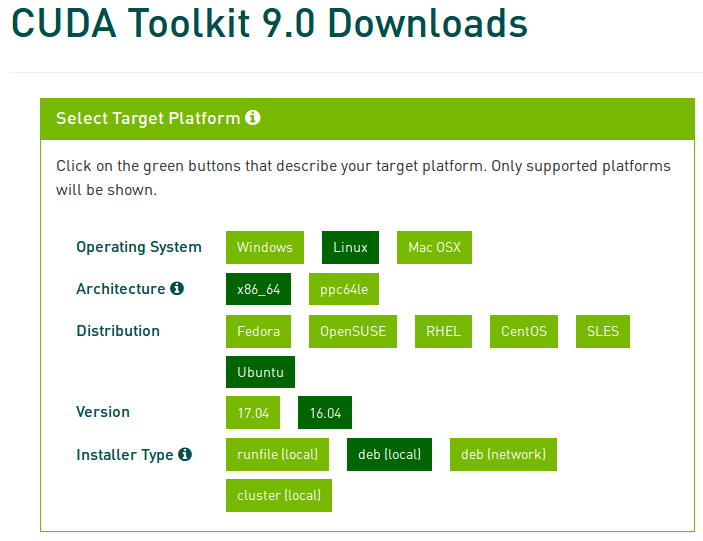
\includegraphics[width=1.1\textwidth]{CUDA_9_0} 
\end{center}
\end{figure}
\vspace{-0.5cm}

共三个deb文件:1为 CUDA 9.0基础安装包,2-3为其更新包。
\begin{itemize}
\item[1.] cuda-repo-ubuntu1604-9-0-local\_9.0.176-1\_amd64.deb(1.2G)
\item[2.] cuda-repo-ubuntu1604-9-0-local-cublas-performance-update\_1.0-1\_amd64.deb(100.2M)
\item[3.] cuda-repo-ubuntu1604-9-0-local-cublas-performance-update-2\_1.0-1\_amd64.deb(100.0M)
\end{itemize}

按照1-2-3的顺序进行安装,先基础安装包,首先在终端切换路径到deb安装包所在路径(cd $\sim$/\emph{<debDirectory>}),然后依次输入如下四行命令:
\begin{itemize}
\item[1.] \$ sudo dpkg -i cuda-repo-ubuntu1604-9-0-local\_9.0.176-1\_amd64.deb
\item[2.] \$ sudo apt-key add /var/cuda-repo-{\color{red}9-0-local}/7fa2af80.pub 
\item[3.] \$sudo  apt-get update
\item[4.] \$ sudo apt-get install cuda
\end{itemize}
注意,第二行命令官网给的是 sudo apt-key add /var/cuda-repo-{\color{red}<version>}/7fa2af80.pub,其中的{\color{red}<version>}是需要我们输入安装的 CUDA 9.0版本号,为便于确定版本号的正确输入形式,大家可以输入这行命令的前一半命令:sudo apt-key add /var/cuda-repo-,然后按{\color{red}Tab}键自动补齐版本号。这里已经给大家确定了其正确的版本号输入形式,直接copy运行即可顺利安装。

接着安装更新包(默认三个deb均在同一路径下),在终端依次输入如下二行命令:
\vspace{-0.2cm}
\begin{itemize}
\item[1.] \$ sudo dpkg -i cuda-repo-ubuntu1604-9-0-local-cublas-performance-update\_1.0-1\_amd64.deb 
\item[2.] \$ sudo dpkg -i cuda-repo-ubuntu1604-9-0-local-cublas-performance-update-2\_1.0-1\_amd64.deb 
\end{itemize}

至此,CUDA 9.0安装完毕。下面进行cuDNN 7.0的下载与安装。



\subsection{ cuDNN 7.0的下载与安装}
进入 \url {https://developer.nvidia.com/rdp/cudnn-archive } 下载与CUDA  9.0版本相匹配的cuDNN版本,这里需要注册账号、登录并进行问卷调查(问卷不多于5个问题)才能下载。本教程下载Download cuDNN v7.0.5 [Dec 5, 2017], for CUDA 9.0 -cuDNN v7.0.5 Library for Linux 进行配置,下载文件为cudnn-9.0-linux-x64-v7.tgz(333M)或是cudnn-9.0-linux-x64-v7.solitairetheme8(348.8M)。

若是下载的cudnn-9.0-linux-x64-v7.tgz压缩文件,先使用如下命令进行解压:
\begin{center}
\$ tar xvf cudnn-9.0-linux-x64-v7.tgz
\end{center}
也可直接右键“提取到此处”,简单粗暴。

若是下载的cudnn-9.0-linux-x64-v7.solitairetheme8文件,先使用如下命令将其转换为tgz文件:
\vspace{-0.2cm}
\begin{center}
\$ cp cudnn-9.0-linux-x64-v7.solitairetheme8  cudnn-9.0-linux-x64-v7.tgz
\end{center}
然后采用上述方法解压,或者直接右键“提取到此处”。当然也可直接将cudnn-9.0-linux-x64-v7.{\color{red}solitairetheme8}的后缀名改为.{\color{red}tgz},然后右“提取到此处”,简单粗暴、疗效快。

在终端依次输入如下三行命令:
\vspace{-0.2cm}
\begin{itemize}
\item[1.] \$ sudo cp cuda/include/cudnn.h  /usr/local/cuda/include
\item[2.] \$ sudo cp cuda/lib64/libcudnn*  /usr/local/cuda/lib64
\item[3.] \$ sudo chmod a+r /usr/local/cuda/include/cudnn.h /usr/local/cuda/lib64/libcudnn*
\end{itemize}

至此,cuDNN 7.0安装完毕。



%libcupti-dev库的安装
\section{libcupti-dev库的安装}
根据\href{https://www.tensorflow.org/install/install_linux}{TensorFlow安装教程说明:}

\emph{The libcupti-dev library, which is the NVIDIA CUDA Profile Tools Interface. This library provides advanced profiling support. To install this library, issue the following command for CDDA Toolkit $\ge$ 8.0:}
\begin{center}
\$ sudo apt-get install cuda-command-line-tools
\end{center}

但是,当你输入上述命令后,你会得到如下的 {  \color{red} {\heiti 错误提示}:
\begin{center}
\emph{
\textbf E: Unable to locate package cuda-command-line-tools
}
\end{center}
}
这是因为{\heiti 没有指定cuda-command-line-tools的版本},那么如何解决呢?经过检索发现,{\color{red}这是TensorFlow Linux安装教程的一个bug},在TensorFlow的github主页下,有人提交了该问题的Issues:\href{https://github.com/tensorflow/tensorflow/issues/16214}{Unable to locate package cuda-command-line-tools}。其中二楼 \href{https://github.com/cyrilzh}{ cyrilzh }给出了一个解决办法:
\begin{center}
\$ sudo apt-cache search cuda-command-line-tool
\end{center}

使用上述命令在源软件列表中查找相应的软件包,此时会返回包含“cuda-command-line-tool”字段的所有cuda-command-line-tools版本。例如搜索结果如下:\\
cuda-command-line-tools-8-0 - CUDA command-line tools\\
cuda-command-line-tools-9-0 - CUDA command-line tools

然后选择相应的版本安装即可。例如本教程安装的是CUDA 9.0,因此选择与之匹配的“{\color{red}cuda-command-line-tools-9-0}”进行安装,命令如下:
\begin{center}
\$ sudo apt-get install cuda-command-line-tools-9-0
\end{center}

当然,上述办法也可使用Tab键的自动补齐功能来辅助查找相应版本,两者有异曲同工之妙。



%环境变量配置
\section{环境变量配置}
在终端依次输入如下命令:
\vspace{-0.2cm}
\begin{center}
\$ sudo gedit ~/.bash\_profile
\end{center}
打开个人配置文件,然后在文件末尾添加下列三行内容(以export开头):
\begin{center}
export LD\_LIBRARY\_PATH="\$LD\_LIBRARY\_PATH:/usr/local/
cuda/lib64:/usr/local/cuda/extras/CUPTI/lib64"

export CUDA\_HOME=/usr/local/cuda

export LD\_LIBRARY\_PATH=/usr/local/cuda/lib64/
\end{center}
保存并退出,然后在终端输入
\vspace{-0.2cm}
\begin{center}
\$ source ~/.bash\_profile
\end{center}
更新当前变量环境。



%测试CUDA 9.0 和cuDNN 7.0的安装情况
\section{测试CUDA 9.0 和cuDNN 7.0的安装情况}
在终端输入如下命令:
\begin{itemize}
\item[1.] \$ cd  /usr/local/cuda-9.0/samples/1\_Utilities/deviceQuery
\item[2.] \$ sudo make
\item[3.] \$ ./deviceQuery
\end{itemize}

\newpage

若显示本机GPU属性信息,如下图所示,则表明上述安装成功。
\begin{figure}[h]
\begin{center}
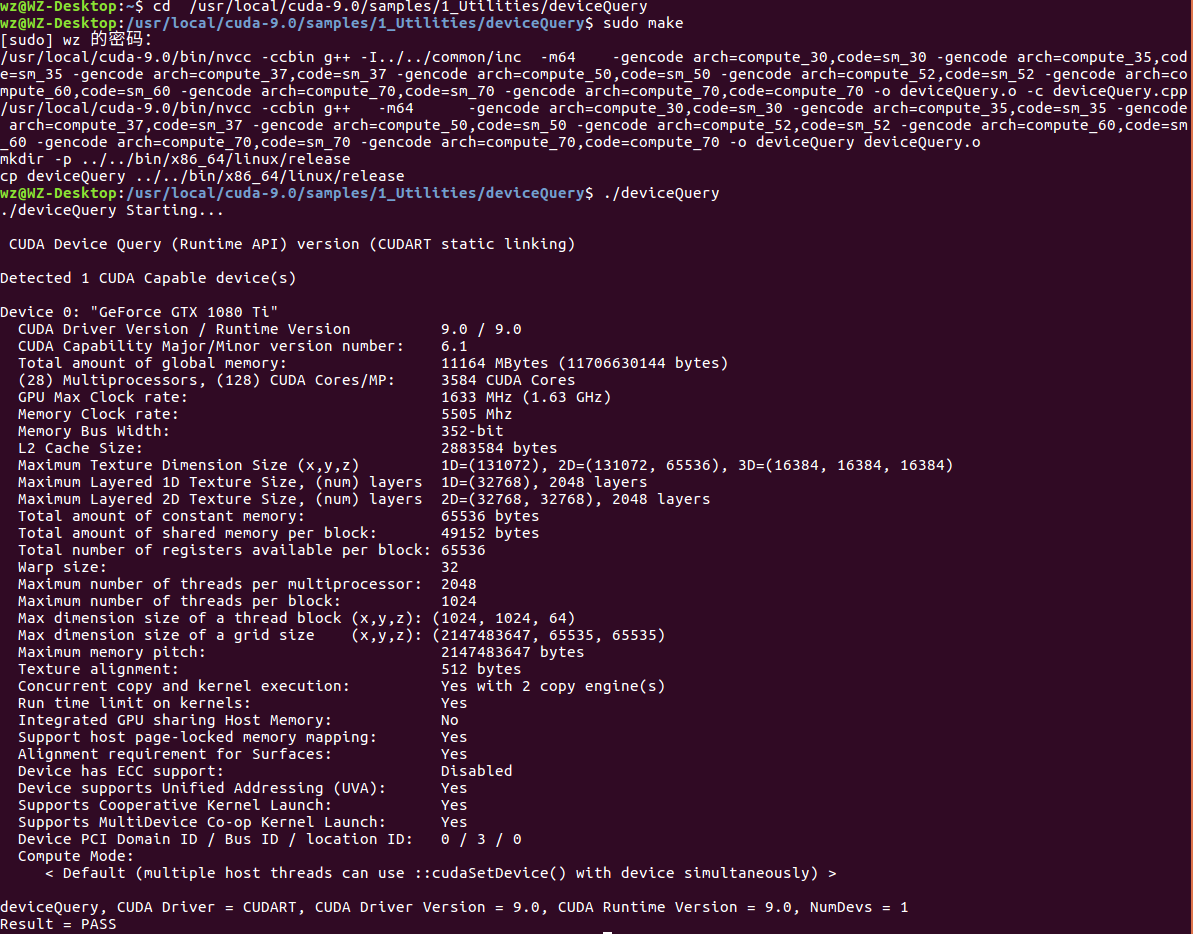
\includegraphics[width=\textwidth]{test1} 
\end{center}
\end{figure}

\vspace{-0.2cm}
\noindent 若出现错误:

CUDA Device Query (Runtime API) version (CUDART static linking)

cudaGetDeviceCount returned 35 

-> CUDA driver version is insufficient for CUDA runtime version 

Result = FAIL

此种情况多是由于笔记本电脑是双显卡(含Intel 集成显卡与NVIDIA显卡)配置,但其NVIDIA显卡没启用所致。解决办法如下,终端输入:
\vspace{-0.2cm}
\begin{center}
\$ nvidia-settings
\end{center}
打开NVIDIA控制面板,在左侧PRIME Profiles项中切换到NVIDIA显卡,然后重启Ubuntu系统即可,再次测试便能成功。



也可在终端再次输入如下命令进行二次测试:
\vspace{-0.2cm}
\begin{itemize}
\item[1.] \$ cd  /usr/local/cuda-9.0/samples/1\_Utilities/bandwidthTest
\item[2.] \$ sudo make
\item[3.] \$ ./bandwidthTest
\end{itemize}


经过以上两次测试,即可验证前述工作初见成效。下面正式开始配置TensorFlow-GPU环境!


%配置TensorFlow-GPU环境
\section{配置TensorFlow-GPU环境}
\href{https://www.tensorflow.org/install/install_linux}{TensorFlow官方安装教程}
提供了五种方式来安装TensorFlow:Virtualenv、“native”pip、Docker、Anaconda以及从源码编译安装,官方推荐使用Virtualenv来进行安装:

\emph{{\textbf {We recommend the Virtualenv installation}}. Virtualenv is a virtual Python environment isolated from other Python development, incapable of interfering with or being affected by other Python programs on the same machine. During the Virtualenv installation process, you will install not only TensorFlow but also all the packages that TensorFlow requires. (This is actually pretty easy.) To start working with TensorFlow, you simply need to ``activate" the virtual environment. All in all, Virtualenv provides a safe and reliable mechanism for installing and running TensorFlow.}

\emph{Native pip installs TensorFlow directly on your system without going through any container system.{\textbf { We recommend the native pip install for system administrators aiming to make TensorFlow available to everyone on a multi-user system}}. Since a native pip installation is not walled-off in a separate container, the pip installation might interfere with other Python-based installations on your system. However, if you understand pip and your Python environment, a native pip installation often entails only a single command.}

\emph{Docker completely isolates the TensorFlow installation from pre-existing packages on your machine. The Docker container contains TensorFlow and all its dependencies. Note that the Docker image can be quite large (hundreds of MBs). You might choose the Docker installation if you are incorporating TensorFlow into a larger application architecture that already uses Docker.}

\emph{In Anaconda, you may use conda to create a virtual environment. However, within Anaconda, we recommend installing TensorFlow with the \emph{pip install} command, not with the \emph{conda install} command.}

\emph{{\textbf {NOTE}}: The conda package is community supported, not officially supported. That is, the TensorFlow team neither tests nor maintains the conda package. Use that package at your own risk.}

下面逐步实现:
\vspace{-0.2cm}
\begin{itemize}
\item[1.] 安装 pip (前面已经完成)和 Virtualenv:\\
\$ sudo apt-get install python3-pip python3-dev python-virtualenv

\item[2.] 创建 Virtualenv环境:\\
\$ virtualenv --system-site-packages -p python3 /home/wz/App/tensorflow

{ \color{red}\emph{注意:路径 /home/wz/App/tensorflow为自己定义,本文设定安装在此路径下,读者根据实际情况做相应修改(下同)。}}
\item[3.] 激活 Virtualenv环境\label{activate}:\\
\$ source /home/wz/App/tensorflow/bin/activate

此时,终端的源命令提示符前部分应标识了“(tensorflow)”字段:\\
 (tensorflow) wz@WZ-Desktop:$\sim$\$ 

\item[4.] 在激活的Virtualenv环境中安装TensorFlow-GPU(当然也可以安装CPU版本的TensorFlow)\\
(tensorflow) wz@WZ-Desktop:$\sim$\$  pip3 install tensorflow-gpu==1.6.0\\
{ \color{red}\emph{注意:\\
1. tensorflow-gpu-1.6.0 版本大约210M,这里配置的是1.6.0版本的tensorflow-gpu,当然CUDA 9.0 和cuDNN 7.0对tensorflow-gpu版本是向下兼容的,也就是说这里也可以安装1.5.0、1.4.0或1.3.0等低版本的tensorflow-gpu。tensorflow-gpu版本之间的切换并无特定要求,具备“回滚”功能,也就是说安装tensorflow-gpu-1.X.0版本的同时会自动卸载tensorflow-gpu-1.Y.0版本(X与Y没有大小、先后之分),可使用上述命令指定安装版本来切换不同的tensorflow-gpu版本,没有后顾之忧。\\
2. 至于最新版的tensorflow-gpu-1.7.0 ,笔者未曾测试,不敢妄下断言,还请读者自证。}}

\end{itemize}

此时终端提示信息如下:\\
Successfully installed absl-py-0.1.11 astor-0.6.2 bleach-1.5.0 gast-0.2.0 grpcio-1.10.0 html5lib-0.9999999 markdown-2.6.11 numpy-1.14.2 protobuf-3.5.2.post1 tensorboard-1.6.0 tensorflow-gpu-1.6.0 termcolor-1.1.0 werkzeug-0.14.1\\
表示 tensorflow-gpu-1.6.0 初步成功安装(也同时安装tensorboard)。


%测试TensorFlow-GPU安装情况
\section{测试TensorFlow-GPU安装情况}

需要注意的是,每次使用TensorFlow的时候,必须\hyperref[activate]{先激活Virtualenv 环境}。\\
测试流程如下:

\noindent (tensorflow) wz@WZ-Desktop:$\sim$\$ python\\
Python 3.5.2 (default, Nov 23 2017, 16:37:01) 

\noindent [GCC 5.4.0 20160609] on linux\\
Type "help", "copyright", "credits" or "license" for more information.\\
> > > import tensorflow as tf\\
> > > a = tf.constant([1.0, 2.0, 3.0, 4.0, 5.0, 6.0], shape=[2, 3], name='a')\\
> > > b = tf.constant([1.0, 2.0, 3.0, 4.0, 5.0, 6.0], shape=[3, 2], name='b')\\
> > > c = tf.matmul(a, b)\\
> > > sess = tf.Session(config=tf.ConfigProto(log\_device\_placement=True))\\
显示如下信息:\\
2018-03-18 17:46:08.206276: I tensorflow/core/common\_runtime/gpu/gpu\_device.cc:1212] Found device 0 with properties: \\
name: GeForce GTX 1080 Ti major: 6 minor: 1 memoryClockRate(GHz): 1.6325\\
pciBusID: 0000:03:00.0\\
totalMemory: 10.90GiB freeMemory: 10.44GiB\\
2018-03-18 17:46:08.206317: I tensorflow/core/common\_runtime/gpu/gpu\_device.cc:1312] Adding visible gpu devices: 0\\
2018-03-18 17:46:08.416506: I tensorflow/core/common\_runtime/gpu/gpu\_device.cc:993] Creating TensorFlow device (/job:localhost/replica:0/task:0/device:GPU:0 with 10104 MB memory)\\ -> physical GPU (device: 0, name: GeForce GTX 1080 Ti, pci bus id: 0000:03:00.0, compute capability: 6.1)\\
Device mapping:\\
/job:localhost/replica:0/task:0/device:GPU:0 -> device: 0, name: GeForce GTX 1080 Ti, pci bus id: 0000:03:00.0, compute capability: 6.1\\
2018-03-18 17:46:08.526242: I tensorflow/core/common\_runtime/direct\_session.cc:297] Device mapping:\\
\\
> > >  print(sess.run(c))
MatMul: (MatMul): /job:localhost/replica:0/task:0/device:GPU:0\\
2018-03-18 17:46:31.856736: I tensorflow/core/common\_runtime/placer.cc:875] MatMul: (MatMul)/job:localhost/replica:0/task:0/device:GPU:0\\
b: (Const): /job:localhost/replica:0/task:0/device:GPU:0\\
2018-03-18 17:46:31.856797: I tensorflow/core/common\_runtime/placer.cc:875] b: (Const)/job:localhost/replica:0/task:0/device:GPU:0\\
a: (Const): /job:localhost/replica:0/task:0/device:GPU:0\\
2018-03-18 17:46:31.856822: I tensorflow/core/common\_runtime/placer.cc:875] a: (Const)/job:localhost/replica:0/task:0/device:GPU:0
\[\begin{bmatrix}
22. &28. \\ 
49. &64. 
\end{bmatrix}\]


到此,即验证了TensorFlow-GPU完全安装成功!

若退出TensorFlow环境,可使用如下命令:
\vspace{-0.2cm}
\begin{center}
(tensorflow) wz@WZ-Desktop:$\sim$\$ deactivate
\end{center}

若卸载TensorFlow,只要移除创建的tensorflow根目录即可,使用如下命令:
\vspace{-0.2cm}
\begin{center}
(tensorflow) wz@WZ-Desktop:$\sim$\$ rm -r /home/wz/App/tensorflow
\end{center}


%常见问题与解决办法
\section{常见问题与解决办法}

一般来说,按照上述流程顺利走下来,TensorFlow-GPU便可以完全配置成功。但有时候也会出现某种“意外”,尤其是当ubuntn安装某些依赖失败导致当前环境紊乱时。

笔者就遇到过这样一个问题:按照上述流程配置CUDA 8.0 + cuDNN6.0 + TensorFlow-GPU 1.4.0,在导入tensorflow时候,提示:\\
{\color{red}\emph{
ImportError: libcublas.so.6.0: cannot open shared object file: No such file or directory
}}

{\heiti 初步分析原因是本地/usr/local/lib缺少cuDNN6.0 的动态连接库文件libcublas.so.6.0(因为cuDNN6.0最高可支持TensorFlow-GPU 1.4.0并向下兼容,cuDNN7.0可支持TensorFlow-GPU 1.6.0并向下兼容,所以排除版本之间不兼容原因;同时相关路径已经添加到系统环境)}。

{\heiti  \color{green}解决办法是将与libcublas.so.6.0(在/usr/local/cuda-8.0/lib64/下)相关的三个文件复制到/usr/local/lib文件夹下(注意与安装的cuda版本号)}:\\
{\textbf {
\$ sudo cp /usr/local/cuda-8.0/lib64/libcudnn.so /usr/local/lib/libcudnn.so \&\& sudo ldconfig\\
\$ sudo cp /usr/local/cuda-8.0/lib64/libcudnn.so.6 /usr/local/lib/libcudnn.so.6 \&\& sudo ldconfig\\
\$ sudo cp /usr/local/cuda-8.0/lib64/libcudnn.so.6.0.21 /usr/local/lib/libcudnn.so.6.0.21 \&\& sudo ldconfig
}}


若读者在按照本教程配置CUDA 9.0 + cuDNN8.0 + TensorFlow-GPU 1.6.0或其他组合时出现类似问题:\\
{\emph{
ImportError: libcublas.so.{\color{red}x}.0: cannot open shared object file: No such file or directory
}}\\
{ \color{red} \heiti 可参照上述方法复制相关文件到/usr/local/lib文件夹下},即可解决问题。



\begin{thebibliography}{99}  
\bibitem{1} \url{https://tensorflow.google.cn/install/install_linux}
\bibitem{2} \url{http://blog.csdn.net/u014696921/article/details/60140264}
\bibitem{3} \url{https://blog.csdn.net/10km/article/details/61665578}
\end{thebibliography}  


\end{document}



